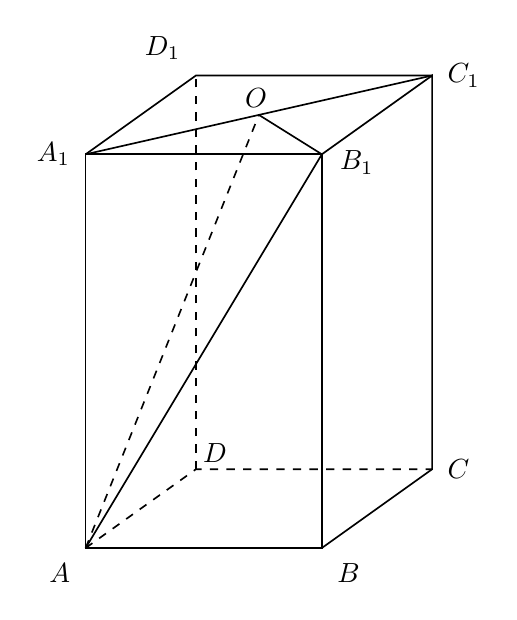
\begin{tikzpicture}[x=1cm,y=1cm,line width=.6pt]
% Long cuboid ABCD-A1B1C1D1, front ABB1A1, depth vector (1.4,1.0)
\coordinate (A) at (0,0);
\coordinate (B) at (3,0);
\coordinate (B1) at (3,5);
\coordinate (A1) at (0,5);
\coordinate (D) at (1.4,1.0);
\coordinate (C) at (4.4,1.0);
\coordinate (D1) at (1.4,6.0);
\coordinate (C1) at (4.4,6.0);
\coordinate (O) at (2.2,5.5);
% solid outer + top
\draw (A) -- (B) -- (B1) -- (A1) -- cycle;
\draw (B) -- (C) -- (C1) -- (B1);
\draw (A1) -- (D1) -- (C1);

\draw (A1) -- (C1);
\draw (A) -- (B1);
\draw (O) -- (B1);
% dashed hidden + interior
\draw[dashed] (A) -- (D) -- (C);
\draw[dashed] (D) -- (D1);
\draw[dashed] (A) -- (O);
% labels offset from points to avoid touching strokes
\node[below left=2pt] at (A) {$A$};
\node[below right=2pt] at (B) {$B$};
\node[right=2pt] at (C) {$C$};
\node[right=1pt,xshift=-2pt,yshift=6pt] at (D) {$D$};
\node[left=2pt] at (A1) {$A_{1}$};
\node[right=2pt,xshift=1.0pt,yshift=-3.0pt] at (B1) {$B_{1}$};
\node[right=2pt] at (C1) {$C_{1}$};
\node[above left=2pt] at (D1) {$D_{1}$};
\node[above=2pt,xshift=-1.0pt,yshift=-3.0pt] at (O) {$O$};
\end{tikzpicture}
